\documentclass[psamsfonts]{amsart}

%-------Packages---------
\usepackage{amssymb,amsfonts}
\usepackage[all,arc]{xy}
\usepackage{enumerate}
\usepackage[margin=1in]{geometry}
\usepackage{amsthm}
\usepackage{theorem}
\usepackage{verbatim}
\usepackage{framed}
\usepackage{tikz}
\usetikzlibrary{shapes,arrows}

\newenvironment{sol}{\vspace{0.25cm}{\large \bfseries Solution:}}{\qedsymbol}
\newenvironment{prob}[1]{\begin{framed}{\large \bfseries Problem #1:}}{\end{framed}}
\newcommand{\makenewtitle}{
    \begin{center}
    {\huge \bfseries 6.854 Advanced Algorithms} \\
    Problem Set 2\\
    \vspace{0.25cm}
    {\bfseries John Wang} \\
    Collaborators:
    \end{center}
    \vspace{0.5cm}
}


\bibliographystyle{plain}

\voffset = -10pt
\headheight = 0pt
\topmargin = -20pt
\textheight = 690pt

%--------Meta Data: Fill in your info------
\title{6.854 \\
Advanced Algorithms \\
Problem Set 4}

\author{John Wang}

\begin{document}

\maketitle

Collaborators: 

\begin{prob}{1-a}
Consider a second-level table, that in the static case uses $f(s) = O(s^2)$ space to store $s$ items. We gave a construction of such a table that succeeds with probability $1/2$. Suppose that we take the following approach to insertions: if inserting the $s$th item violates perfection of the table, repeatedly build a table of size $f(2s)$ until you get a perfect one. Show that when $s$ items are inserted (one at a time, with rebuilds as necessary) the expected total cost of all the rebuilds is $O(s)$. 
\end{prob}

\begin{sol}

\end{sol}

\newpage 
\makenewtitle

\begin{prob}{2-a}
In any maximum flow, and for all vertices $v$ and $w$, either the raw flow from $v$ to $w$ or the raw flow from $w$ to $v$ is 0.
\end{prob}
\begin{sol}
False. Consider the following graph.

\begin{figure}[h!]
\centering
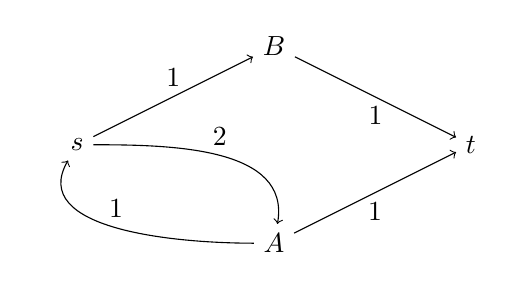
\begin{tikzpicture}[scale=2.5]
\node (s) at (0,0.5) {$s$};
\node (A) at (1,0) {$A$};
\node (B) at (1,1) {$B$};
\node (t) at (2,0.5) {$t$};
\path[->,font=\scriptsize,>=angle 90];
\draw (s) edge [->,relative=false,in=80,out=0] node[above]{2} (A)
(A) edge [->,relative=false,in=-120,out=-180] node[above]{1} (s)
(s) edge [->] node[above]{1} (B)
(B) edge [->] node[below]{1} (t)
(A) edge [->] node[below]{1} (t);
\end{tikzpicture}
\end{figure}

It is clear that the maximum flow is 2, where flow comes into $t$ from nodes $A$ and $B$, each with a flow of 1. However, we can see that there is non-zero raw flow from $s$ to $B$ and from $B$ to $s$. Thus, there is a maximum flow where there exist two vertices $v$ and $w$ which break the above conjecture.
\end{sol}

\begin{prob}{2-b}
There always exists a maximum flow such that, for all vertices $v$ and $w$, either the raw flow from $v$ to $w$ or the raw flow from $w$ to $v$ is zero.
\end{prob}

\begin{sol}
True. We will show this by contradiction. Suppose this is not the case. Then there is raw flow such that on some vertices $v$ and $w$, the raw flow from $v$ to $w$ and from $w$ to $v$ are nonzero for all flows which are maximal. This means that any flow with zero raw flow in each direction is not a maximum flow (of flow $f$), so that this new flow would be less than $f$. Now, consider what happens when we set the raw flow from $w$ to $v$ to be zero, and the raw flow from $v$ to $w$ to be $rf(v,w) - rf(w,v)$ where $rf$ denotes raw flow. In this way, we have created a graph $G'$ which has the same amount of flow as before towards the sink (if not, the switch $v$ and $w$) as in the original graph. This means that the new flow is also a maximum flow. However, we know that the flow on the vertices of the rest of the graph are unchanged, and we also assumed that there does not exist any maximum flow with zero raw flow between any vertices $v$ and $w$. This is a contradiction.
\end{sol}

\begin{prob}{2-c}
If all directed edges in a network have distinct capacities, then there is a unique maximum flow.
\end{prob}

\begin{sol}
False. Consider the following counterexample.
\begin{figure}[h!]
\centering
\begin{tikzpicture}[scale=2.5]
\node (v0) at (0,0) {$s$};
\node (v1) at (1,0) {$A$};
\node (v2) at (3,0) {$t$};
\node (v3) at (2,0.5) {$B$};
\path[->,font=\scriptsize,>=angle 90];
\draw (v0) edge [->] node[below]{1} (v1)
(v1) edge [->] node[below]{3} (v2)
(v1) edge [->] node[above]{2} (v3)
(v3) edge [->] node[above]{4} (v2);
\end{tikzpicture}
\end{figure}

In the graph above, the maximum possible flow is $F = 1$. However, there are two possible ways that this flow can be achieved. In the first case, a flow of capacity 1 can move along the path $S, A, t$. In the second case, a flow of capacity 1 can move along the path $S, A, B, t$.
\end{sol}

\begin{prob}{2-d}
If we replace each directed edge in a network with two directed edges in opposite directions with the same capacity and connecting the same vertices, then the value of the maximum flow remains unchanged.
\end{prob}

\begin{sol}
False. Consider the simple graph with two nodes $s$ and $t$. The only edge in this graph is a directed edge from $t$ to $s$ of capacity $v$. Clearly, the maximum flow from $s$ to $t$ is zero, because there is no way to reach $t$. However, if we augment the graph with two edges in opposite directions, both of capacity $v$, then the maximum flow becomes $v$.
\end{sol}

\begin{prob}{2-e}
If we add the same positive number $\lambda$ to the capacity of every directed edge, then the minimum cut (but not its value) remains unchanged.
\end{prob}

\begin{sol}
False. Consider the graph below. 
\begin{figure}[h!]
\centering
\begin{tikzpicture}[scale=2.5]
\node (s) at (0,0) {$s$};
\node (A) at (1,0) {$A$};
\node (B) at (2,0.5) {$B$};
\node (C) at (2,-0.5) {$C$};
\node (t) at (3,0) {$t$};
\path[->,font=\scriptsize,>=angle 90];
\draw (s) edge [->] node[below]{5} (A)
(A) edge [->] node[above]{3} (B)
(A) edge [->] node[below]{2} (C)
(C) edge [->] node[below]{10} (t)
(B) edge [->] node[above]{10} (t);
\end{tikzpicture}
\end{figure}

We see that on the original graph, the unique $s-t$ cut is given by $S = \{s, A, B, C\}$ and $T = \{t\}$. However, when $\lambda = 1$ is added to all of the edge capacities, we see that the new unique $s-t$ cut is given by $S = \{s\}$ and $T = \{A, B, C, t \}$, since the bottleneck appears at $A$ when its capacity is only increased by 1, and the capacities of both outgoing edges are both increased by 1, leading to a total increase of 2. 
\end{sol}

\begin{prob}{2-f}
Flow is transitive: if in a graph there is a flow of value $v$ from $s$ to $t$ and there is a flow of value $v$ from $t$ to $u$, then there is a flow of value $v$ from $s$ to $u$.
\end{prob}
\begin{sol}
False. Consider the following graph:
\begin{figure}[h!]
\centering
\begin{tikzpicture}[scale=2.5]
\node (s) at (0,0) {$s$};
\node (t) at (3,0) {$t$};
\node (u) at (1.5,0.45) {$u$};
\path[->,font=\scriptsize,>=angle 90];
\draw (s) edge node[below]{1} (t)
(t) edge node[above]{1} (u)
(s) edge node[above]{4} (u);
\end{tikzpicture}
\end{figure}

From $s$ to $t$, there is a maximum flow of 1. From $t$ to $u$ there is a maximum flow of $1$. However, from $s$ to $u$, there is a maximum flow of 5. Thus, it is clear that the flow from $s$ to $u$ is not equal to the flow from $s$ to $t$ then from $t$ to $u$, since there are other paths for the flow to travel on. 
\end{sol}

\newpage
\makenewtitle

\begin{prob}{5-a}
Argue that the running time of Dial's algorithm is $O(m+D)$ where $D$ is the maximum distance, and that the algorithm still works if some edges have length 0.
\end{prob}
\begin{sol}
First we will initialize an array storing the keys from 1 to $nC$. We know that this can be done in $O(1)$ time. Next, we will perform Dijkstra's algorithm by successively finding the minimum element in the queue, and expanding its neighbors, and decreasing the key by storing the reduced edge lengths $l_{vw}^d = l_{vw} + d_v - d_w$. The total reduced edge length along a path from the source to some node $t$ is $\sum_{v,w} l_{vw}^d$ where $v$ and $w$ are intermediate nodes on the path. Since this sum telescopes, we see that the total reduced edge length is simply $d_t$. This implies that removing the lowest reduced edge length will remove the current shortest path to some node and will not affect the correctness of Dijkstra's.

This means that we can perform $n$ inserts, $n$ delete-mins, and $m$ decrease-keys. We know the insert and decrease key operations cost $O(1)$ each. The delete-min operations cost $O(k)$ where $k$ is the distance between the last minimum and the next minimum (since we have to crawl our way up $k$ buckets until we find the minimum). This means that the total amount of work performed is just $\sum_{i=1}^n k_i$ where $k_i$ is the distance between the minimums at the $i-1$st and $i$th steps. This comes out to the maximum distance, which is $D$. Thus total work is just $O(m + D)$. 

The algorithm clearly still works for edge length of zero because we can initialize a bucket for edges of length 0, which will then always be the minimum in the set, so they will be picked first.
\end{sol}

\begin{prob}{5-b}
Show that the reduced edge lengths defined above are all nonnegative integers.
\end{prob}
\begin{sol}
We need to show that $l_{vw}^d = l_{vw} + d_v - d_w$ are all nonnegative. We know that $d_v, d_w$ and $l_{vw}$ are all nonnegative. Therefore, all we need to do is to show that $l_{vw} \geq d_v - d_w$. Let $\{s, v_1, v_2, \ldots, v\}$ be the shortest path from $s$ to $v$ with distance $d_v$. We know that $d_v + l_{vw} \leq d_{w}$ since the shortest path to $w$ from $s$ puts a lower bound on the distance of any path to $w$ from $s$. This expression rearranges to $l_{vw} \geq d_v - d_w$ which is what we wanted to show.
\end{sol}

\begin{prob}{5-c}
Show that the shortest paths under the reduced length function are the same as those under the original length function. What is the length of shortest paths under $l^d$?
\end{prob}
\begin{sol}
Suppose by contradiction that under the reduced length function, there is some path $P'$ from $s$ to $u$ which is shorter than $P$, where $P$ is the shortest path under the original length function. Let $P = \langle s=v_1, v_2, v_3, \ldots, u=v_n \rangle$ of length $n$ and $P' = \langle s=v'_1, v'_2, v'_3, \ldots, u = v'_{n'}\rangle$ of length $n'$. If $P'$ is shorter than $P$ under the reduced length function, then the following is true:
\begin{eqnarray}
\sum_{i=1}^{n'} l^d_{v_{i-1}' v_{i}'} &<& \sum_{i=1}^n l^d_{v_{i-1} v_i} \\
\sum_{i=1}^{n'} l_{v_{i-1}' v_{i}'} - d_{v'_i} + d_{v'_{i-1}} &<& \sum_{i=1}^{n} l_{v_{i-1} v_{i}} - d_{v_i} + d_{v_{i-1}} \\
-d_{u} + \sum_{i=1}^{n'} l_{v_{i-1}' v_i'} &<& -d_u + \sum_{i=1}^n l_{v_{i-1} v_i} \\
\sum_{i=1}^{n'} l_{v_{i-1}' v_i'} &<& \sum_{i=1}^n l_{v_{i-1} v_i} 
\end{eqnarray}

This occurs because $d_{v_i} - d_{v_{i-1}}$ leads to a telescoping sum. However, this means that path $P'$ has a shorter length than $P$ under the original length function, which is a contradiction of the fact that $P$ was the shortest path under the original length function. Thus, the shortest path under the reduced length function is the same as the one under the original length function.

The length of the shortest paths under $l^d$ is therefore $-d_u + \sum_{i=1}^n l_{v_{i-1} v_{i}}$ where $d_u$ is the distance of the shortest path under the original length function. Thus, the shortest path under the reduced length function is just 0. 
\end{sol}

\begin{prob}{5-d}
Devise a scaling algorithm for shortest paths. Use the reduced edge lengths and Dial's bucketing algorithm to keep the task of shifting in a new bit sample.
\end{prob}
\begin{sol}

\end{sol}
\end{document}
